\SubProblem
{تفاوت \lr{TDD} و \lr{FDD}}
{
در
\lr{Frequency Division Duplexing}
ارتباط دو جهتی در کانال ارتباطی با در نظر گرفتن دو فرکانس متفاوت برای پیوندهای
\lr{Up-link}
و
\lr{Down-link}
صورت می‌گیرد.
این دو پیوند می‌توانند همزمان داده را در دو جهت انتقال دهند پس یک روش
\lr{Full-Duplex}
است.

\begin{itemize}
    \item
    ارسال و دریافت یه صورت همزمان در دو فرکانس متفاوت صورت می‌گیرد و رفتار فرکانسی کانال در این دو جهت متفاوت است.
    
    \item
    ظرفیت دو پیوند فراسو و فروسو ثابت است زیرا فرکانس مشخصی به هر کدام داده شده است و امکان تغییر ظرفیت به صورت پویا وجود ندارد.
    
    \item
    نیازمند باند محافظ
    \lr{(Guard Band)}
    است تا از تداخل فرکانس دو پیوند جلوگیری کند.
    
    \item
    نیازمند
    \lr{Diplexer}
    پیچیده است و در کل روش پیچیده‌تری نسبت به روش زمانی است.

    \item
    استفاده از این روش در کنار روش
    \lr{MIMO}
    بسیار پیچیده است.
    
    \item
    استفاده از این روش در آنتن‌های خاص منظوره پیچیده است.
\end{itemize}

\begin{figure}[H]
    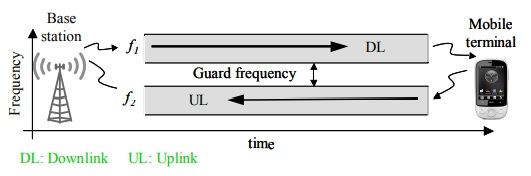
\includegraphics[width=12cm]{Images/FDD.jpg}
    \centering
    \caption{\lr{FDD}}
\end{figure}

در
\lr{Time Division Duplexing}
ارتباط در کانال دیگر با در نظر گرفتن دو فرکانس متفاوت صورت نمی‌گیرد بلکه هر دو پیوند دارای یک باند فرکانسی هستند. استفاده این دو پیوند از این کانال در زمان‌های متفاوت صورت می‌گیرد.
دو پیوند فروسو و فراسو نمی‌توانند در یک زمان و به صورت همزمان از کانال استفاده کنند و زمان‌های مشخصی برای هر پیوند در نظر گرفته شده است پس یک روش
\lr{Half-Duplex}
است.
از این روش می‌توان به صورت همگام
\lr{(Synchronous)}
و ناهمگام
\lr{(Asynchronous)}
استفاده کرد.

\begin{itemize}
    \item
    فرکانس دو پیوند یکسان است، پس رفتار فرکانسی کانال یکسان است.
    
    \item
    نسبت ظرفیت دو پیوند را می‌توان به صورت پویا تغییر داد و به بهره‌وری بهتری رسید.
    
    \item
    نیازمند دوره تناوب محافظ
    \lr{(Guard Period)}
    است تا از تداخل زمانی دو پیوند جلوگیری کند.
    
    \item
    نیازمند
    \lr{Diplexer}
    ساده‌تری است و در کل روش ساده‌تری نسبت به روش فرکانسی است.
    
    \item
    هزینه ساخت و پیاده‌سازی کمتری دارد.

    \item
    نیازمند زمان‌بندی و هماهنگی دقیق است تا اسلات‌های زمانی با هم تداخل نداشته باشند و همچنین کانال بیکار نماند.
    
    \item
    استفاده از این روش در آنتن‌های خاص منظوره ساده‌تر است.
    
    \item
    هم به صورت متقارن و هم نامتقارن می‌توان آن را پیاده‌سازی نمود.
\end{itemize}

\begin{figure}[H]
    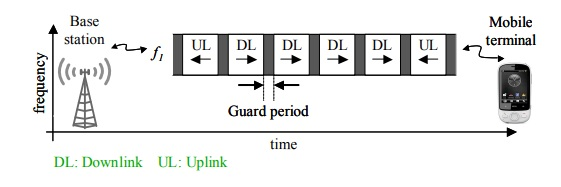
\includegraphics[width=12cm]{Images/TDD.jpg}
    \centering
    \caption{\lr{TDD}}
\end{figure}
}